\documentclass[11pt,a4paper]{article}

\usepackage[utf8]{inputenc}
\usepackage[T1]{fontenc}
\usepackage[french]{babel}
\usepackage{amsmath, amssymb}
\usepackage{graphicx}
\usepackage{geometry}
\usepackage{hyperref}
\usepackage{booktabs}
\usepackage{float}
\usepackage{listings}
\usepackage{xcolor}

\geometry{margin=2.5cm}

\lstset{
  language=R,
  basicstyle=\small\ttfamily,
  keywordstyle=\color{blue!70},
  commentstyle=\color{gray}\itshape,
  stringstyle=\color{orange!80!black},
  breaklines=true,
  frame=single,
  backgroundcolor=\color{gray!8},
  rulecolor=\color{gray!30},
  showstringspaces=false,
  tabsize=2
}

\title{Projet Régression Linéaire \\ \large Polytech Nice Sophia -- MAM3}
\author{Evrard Lecureur, Romain Ben, Thibaud [Nom]}
\date{\today}

\begin{document}

\maketitle

\section*{Introduction}
L'objectif de ce projet est d'étudier la régression linéaire sur plusieurs jeux de données, chacun ayant sa difficulté propre. On a choisi de traiter chaque cas une première fois nous-mêmes, avec ce qu'on connaît du cours (niveau bac+3), puis de regarder ce qu'une IA proposait sur le même problème. L'idée n'est pas de dire qu'une méthode est meilleure que l'autre, mais de voir concrètement ce que l'IA apporte en plus de notre raisonnement.

\tableofcontents

\newpage

%======================================================================
\section{Régression linéaire simple}
%======================================================================

On traite ici quatre jeux de données ($A$, $B$, $C$, $D$). Chacun correspond à une situation différente : un cas qui marche bien, un cas avec des points aberrants, un petit échantillon, et une relation qui n'est pas une droite. Pour chaque jeu, on donne d'abord notre démarche puis ce que l'IA ajoute.

%----------------------------------------------------------------------
\subsection{Rappels}
%----------------------------------------------------------------------

Le modèle de régression linéaire simple s'écrit
\[
Y_i = a X_i + b + U_i, \qquad i = 1, \dots, n,
\]
avec les $U_i$ indépendants et de loi $\mathcal{N}(0, \sigma^2)$. Les estimateurs des moindres carrés sont
\[
\hat{a} = \frac{\sum_{i} (X_i - \bar{X})(Y_i - \bar{Y})}{\sum_{i} (X_i - \bar{X})^2}, \qquad \hat{b} = \bar{Y} - \hat{a}\bar{X}.
\]
Sous les hypothèses du modèle, la statistique $T = \hat{a}/\widehat{\mathrm{SE}}(\hat{a})$ suit une loi de Student à $n-2$ degrés de liberté sous $H_0 : a = 0$. Pour vérifier que le modèle tient, on regarde les résidus studentisés (graphique résidus vs valeurs ajustées et QQ-plot), et on fait un test de Kolmogorov-Smirnov contre la loi $\mathcal{T}(n-3)$.

%----------------------------------------------------------------------
\subsection{Dataset A : cas idéal}
%----------------------------------------------------------------------

\subsubsection{Notre démarche}

On ajuste le modèle avec \texttt{lm()} et on regarde le \texttt{summary()}. Le $R^2$ est très proche de 1 et la p-valeur de la pente est inférieure à $2\cdot10^{-16}$, donc $\hat{a}$ est très significatif. Le nuage de points avec la droite (figure~\ref{fig:A_droite}) confirme que les points sont bien alignés.

\begin{lstlisting}
modele_A <- lm(Y ~ X, data = A)
summary(modele_A)
plot(A$X, A$Y, main = "Dataset A")
abline(modele_A, col = "red")
\end{lstlisting}

\begin{figure}[H]
    \centering
    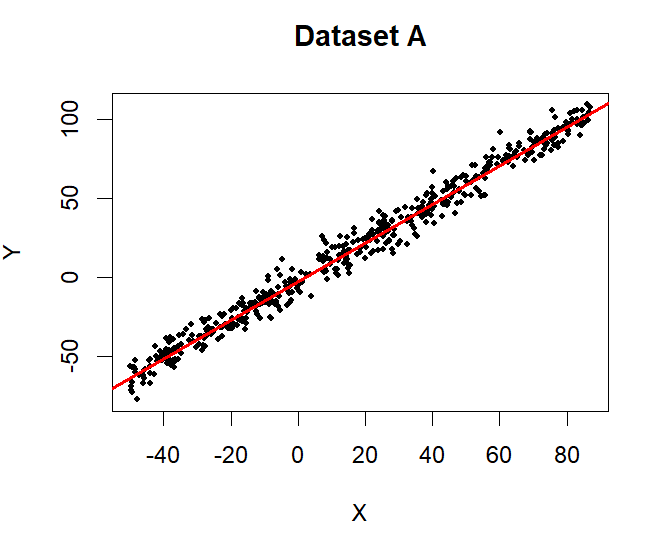
\includegraphics[width=0.7\textwidth]{figures/NuagePointA-droiteRegressionLineaire.png}
    \caption{Dataset A : nuage de points et droite ajustée.}
    \label{fig:A_droite}
\end{figure}

Pour vérifier les hypothèses, on trace les résidus studentisés en fonction des valeurs ajustées, puis le QQ-plot (figure~\ref{fig:A_residus}). Sur le premier graphe les points sont répartis autour de 0 sans forme particulière, donc la variance a l'air constante. Sur le QQ-plot ils suivent à peu près la droite, donc les résidus ont l'air de suivre une loi normale.

\begin{lstlisting}
plot(fitted(modele_A), rstudent(modele_A))
abline(h = 0)
qqnorm(rstudent(modele_A))
qqline(rstudent(modele_A))
\end{lstlisting}

\begin{figure}[H]
    \centering
    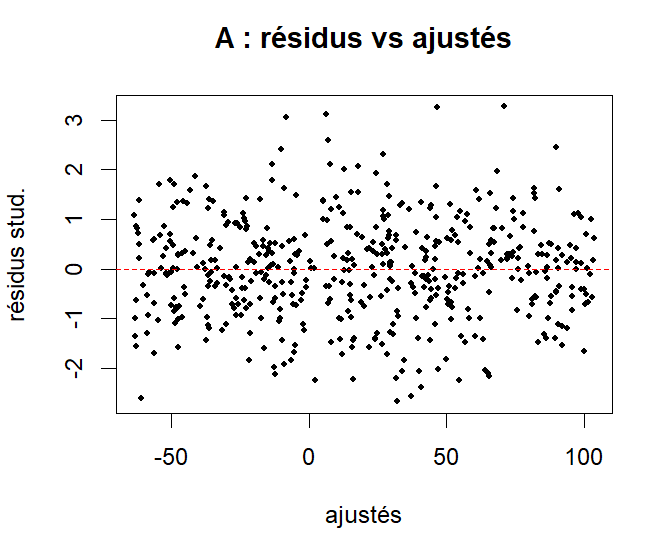
\includegraphics[width=0.48\textwidth]{figures/residuStudent-A.png}
    \hfill
    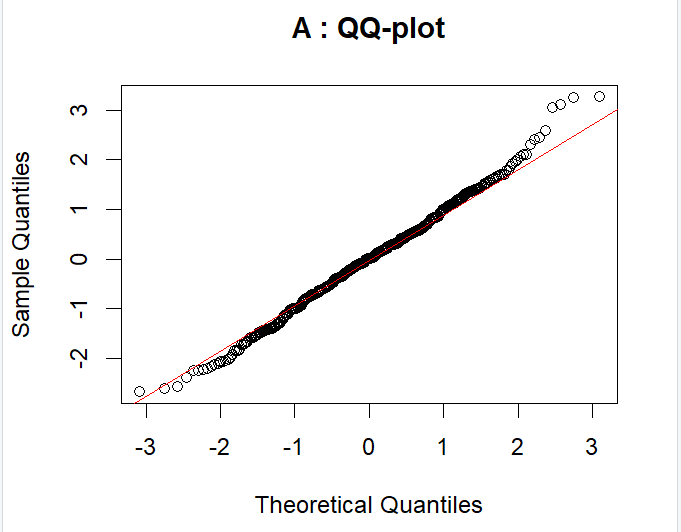
\includegraphics[width=0.48\textwidth]{figures/QQ-plotA.png}
    \caption{Résidus studentisés et QQ-plot, Dataset A.}
    \label{fig:A_residus}
\end{figure}

On confirme avec un test de Kolmogorov-Smirnov des résidus contre une loi de Student à $n-3$ degrés de liberté :

\begin{lstlisting}
n_A <- nrow(A)
ks.test(rstudent(modele_A), "pt", df = n_A - 3)
\end{lstlisting}

La p-valeur est bien au-dessus de 0,05, donc on ne rejette pas la normalité. Les hypothèses sont vérifiées, et le test de Student du \texttt{summary()} nous donne directement que la pente est significative.

\subsubsection{Apport de l'IA}

\begin{itemize}
    \item \textbf{Vérification des formules à la main.} L'IA recalcule $\hat{a}$ et $\hat{b}$ avec les formules du cours pour confirmer ce que renvoie \texttt{summary()}.

\begin{lstlisting}
x_bar <- mean(A$X); y_bar <- mean(A$Y)
a_chap <- sum((A$X - x_bar) * (A$Y - y_bar)) / sum((A$X - x_bar)^2)
b_chap <- y_bar - a_chap * x_bar
cat("calcul manuel -> a =", a_chap, "| b =", b_chap, "\n")
\end{lstlisting}

    \item \textbf{Tests formels en plus.} En complément des graphiques, l'IA ajoute le test de Breusch-Pagan (homoscédasticité) et le test de Shapiro-Wilk (normalité), ce qui donne une conclusion chiffrée et pas seulement visuelle.

\begin{lstlisting}
library(lmtest)
bptest(modele_A)
shapiro.test(residuals(modele_A))
\end{lstlisting}

    \item \textbf{Région de rejet du test.} L'IA trace la densité de Student avec la région de rejet remplie en rouge, ce qui rend la procédure du test plus parlante (figure~\ref{fig:A_rejet}).

\begin{lstlisting}
sigma_chap <- sqrt(sum(residuals(modele_A)^2) / (n_A - 2))
se_a  <- sigma_chap / sqrt(sum((A$X - x_bar)^2))
t_obs <- a_chap / se_a
seuil <- qt(0.975, df = n_A - 2)

curve(dt(x, df = n_A - 2), from = -5, to = 5, n = 500,
      xlab = "t", ylab = "densite", main = "A - region de rejet")
xd <- seq(seuil, 5, length.out = 100)
xg <- seq(-5, -seuil, length.out = 100)
polygon(c(seuil, xd, 5),   c(0, dt(xd, n_A-2), 0), col = rgb(1,0,0,0.3), border = NA)
polygon(c(-5, xg, -seuil), c(0, dt(xg, n_A-2), 0), col = rgb(1,0,0,0.3), border = NA)
abline(v = c(-seuil, seuil), col = "red", lty = 2)
\end{lstlisting}

    \item \textbf{Intervalle de prédiction.} Enfin l'IA utilise \texttt{predict()} avec \texttt{interval = "prediction"} pour encadrer une nouvelle observation.

\begin{lstlisting}
predict(modele_A, newdata = data.frame(X = c(0, 50)), interval = "prediction")
\end{lstlisting}

\end{itemize}

\begin{figure}[H]
    \centering
    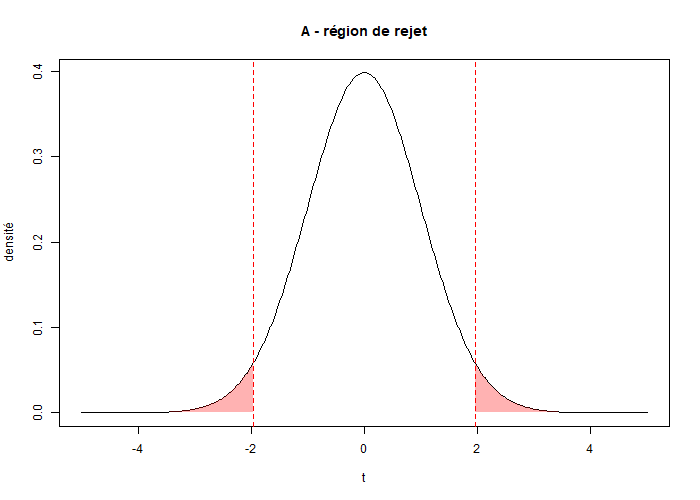
\includegraphics[width=0.65\textwidth]{figures/RegionRejetA.png}
    \caption{Région de rejet du test bilatéral sur la pente, Dataset A.}
    \label{fig:A_rejet}
\end{figure}

%----------------------------------------------------------------------
\subsection{Dataset B : points aberrants}
%----------------------------------------------------------------------

\subsubsection{Notre démarche}

Quand on ajuste le modèle, le $R^2$ est correct, mais le graphique des résidus studentisés (figure~\ref{fig:B_residus}, gauche) montre plusieurs points avec un résidu dont la valeur absolue dépasse 3. Le QQ-plot décroche aux extrémités (figure~\ref{fig:B_residus}, droite) et le test KS rejette la normalité. Il y a donc des points aberrants.

\begin{figure}[H]
    \centering
    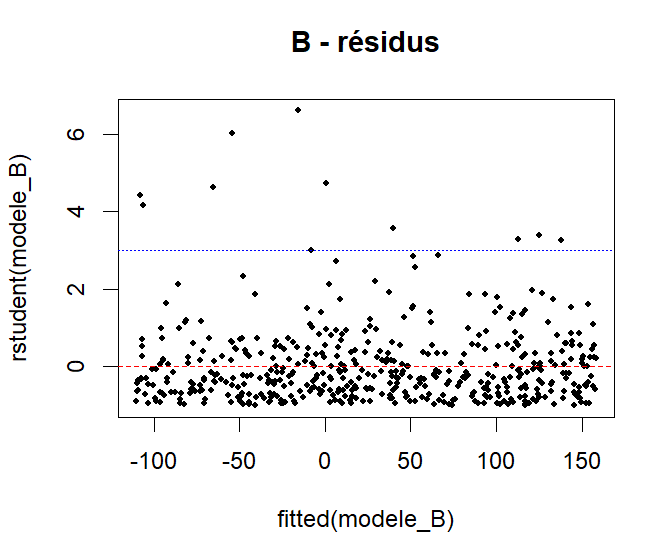
\includegraphics[width=0.48\textwidth]{figures/residuStudent-B.png}
    \hfill
    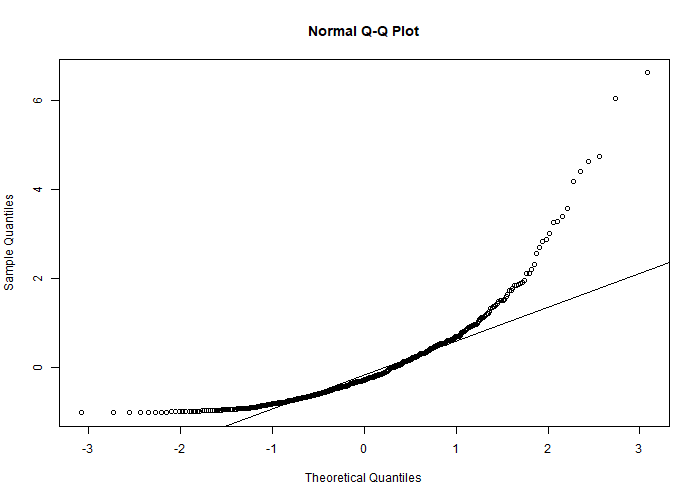
\includegraphics[width=0.48\textwidth]{figures/QQplot-B.png}
    \caption{Résidus et QQ-plot du modèle initial, Dataset B.}
    \label{fig:B_residus}
\end{figure}

On repère ces points avec le critère $|\text{résidu studentisé}| > 3$, on les marque en rouge sur le nuage (figure~\ref{fig:B_outliers}, gauche), puis on refait la régression sans eux (figure~\ref{fig:B_outliers}, droite).

\begin{lstlisting}
out <- which(abs(rstudent(modele_B)) > 3)
plot(B$X, B$Y, main = "outliers")
points(B$X[out], B$Y[out], col = "red")

B2 <- B[-out, ]
modele_B2 <- lm(Y ~ X, data = B2)
coef(modele_B)[2]
coef(modele_B2)[2]
\end{lstlisting}

Après nettoyage, le QQ-plot et le test KS sont bons. La pente a changé entre les deux modèles, ce qui montre bien que les moindres carrés sont sensibles aux valeurs extrêmes.

\begin{figure}[H]
    \centering
    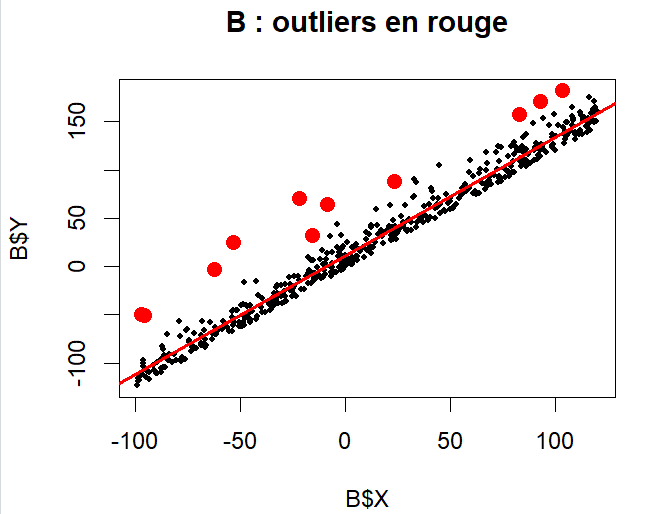
\includegraphics[width=0.48\textwidth]{figures/nuagePointOutliersRouge-B.png}
    \hfill
    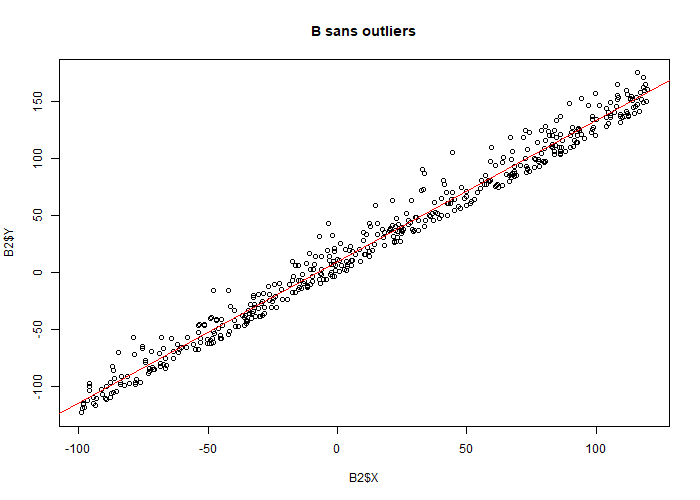
\includegraphics[width=0.48\textwidth]{figures/NuagePointB-nettoye.png}
    \caption{Points aberrants (en rouge) et modèle après retrait, Dataset B.}
    \label{fig:B_outliers}
\end{figure}

\subsubsection{Apport de l'IA}

\begin{itemize}
    \item \textbf{Distance de Cook.} L'IA introduit la distance de Cook pour faire la différence entre un point simplement aberrant (gros résidu) et un point influent (qui tire vraiment les coefficients). Les deux ne sont pas forcément les mêmes.

\begin{lstlisting}
cook_B <- cooks.distance(modele_B)
plot(cook_B, type = "h", main = "B - distance de Cook")
abline(h = 4 / nrow(B), col = "red", lty = 2)
\end{lstlisting}

    \item \textbf{Régression robuste.} Au lieu de supprimer des points, \texttt{rlm()} (package \texttt{MASS}) leur donne automatiquement moins de poids selon leur résidu. On évite ainsi de décider à la main quels points enlever.

\begin{lstlisting}
library(MASS)
modele_B_rob <- rlm(Y ~ X, data = B)
cat("MCO :", coef(modele_B)[2],
    "| rlm :", coef(modele_B_rob)[2],
    "| sans outliers :", coef(modele_B2)[2], "\n")
\end{lstlisting}

    \item \textbf{Comparaison des trois pentes} sur le même graphique (figure~\ref{fig:B_IA}, droite).

\end{itemize}

\begin{figure}[H]
    \centering
    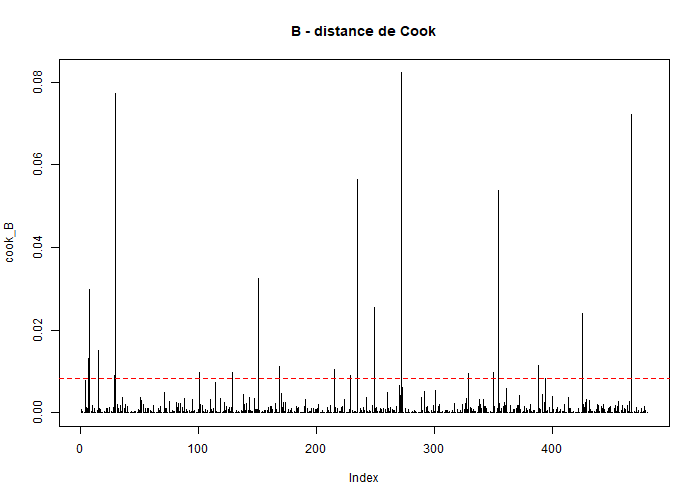
\includegraphics[width=0.48\textwidth]{figures/DistanceCook-B.png}
    \hfill
    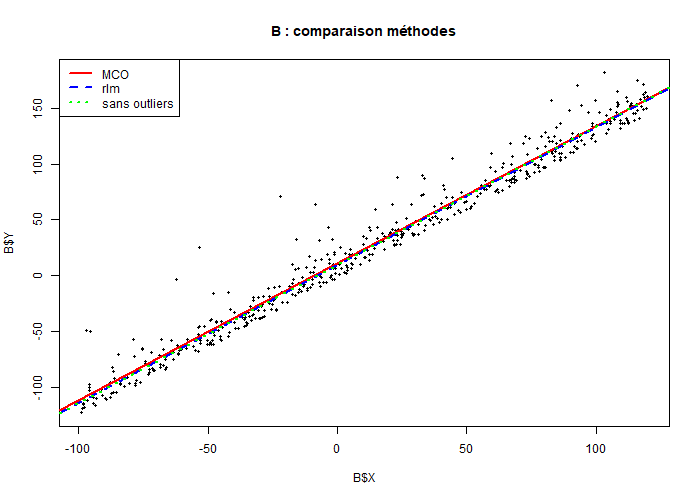
\includegraphics[width=0.48\textwidth]{figures/MCO-rlm-noOutliers-B.png}
    \caption{Distance de Cook et comparaison MCO / rlm / sans outliers, Dataset B.}
    \label{fig:B_IA}
\end{figure}

%----------------------------------------------------------------------
\subsection{Dataset C : petit échantillon ($n = 50$)}
%----------------------------------------------------------------------

\subsubsection{Notre démarche}

Le modèle s'ajuste sans souci et les hypothèses ont l'air vérifiées sur les graphiques (figure~\ref{fig:C_main}). Par contre, en lisant le \texttt{summary()}, on voit que l'erreur standard de la pente est bien plus grande que pour le Dataset A. L'intervalle de confiance à 95\% est donc beaucoup plus large, ce qui est logique vu que la précision se dégrade en $1/\sqrt{n}$ et qu'on a ici beaucoup moins de points.

\begin{lstlisting}
modele_C <- lm(Y ~ X, data = C)
summary(modele_C)$coefficients[2, 2]
confint(modele_C)
\end{lstlisting}

\begin{figure}[H]
    \centering
    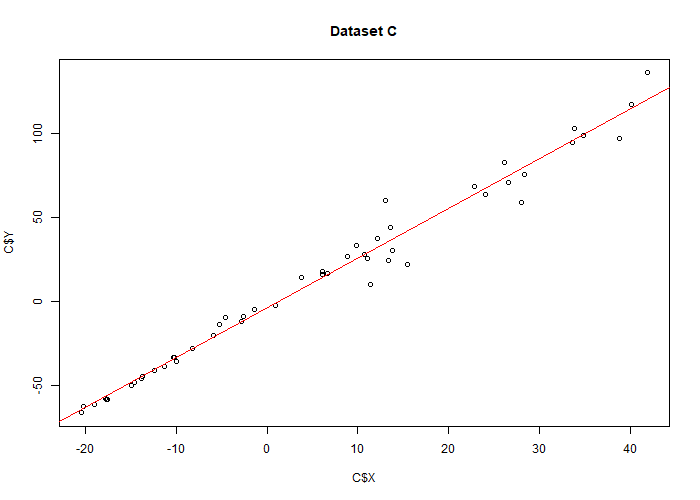
\includegraphics[width=0.48\textwidth]{figures/NuagePointC-DroiteRegression.png}
    \hfill
    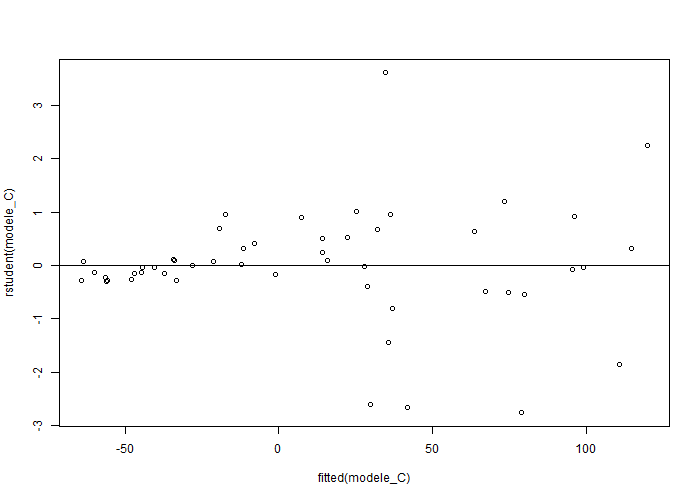
\includegraphics[width=0.48\textwidth]{figures/ResiduStudent-C.png}
    \caption{Ajustement et résidus, Dataset C ($n = 50$).}
    \label{fig:C_main}
\end{figure}

\subsubsection{Apport de l'IA}

\begin{itemize}
    \item \textbf{Tests formels.} En petit échantillon les graphiques sont peu fiables, donc l'IA s'appuie sur le test de Breusch-Pagan pour confirmer l'homoscédasticité.

    \item \textbf{Erreurs standards robustes (sandwich).} En cas de doute, \texttt{vcovHC()} donne une variance robuste des coefficients. C'est un outil classique en économétrie qu'on ne voit pas en cours.

\begin{lstlisting}
library(lmtest); library(sandwich)
bptest(modele_C)
coeftest(modele_C, vcov = vcovHC(modele_C, type = "HC1"))
\end{lstlisting}

    \item \textbf{Bootstrap pour l'intervalle de confiance.} Avec $n = 50$, l'IA propose un bootstrap ($R = 2000$ rééchantillonnages) pour un intervalle qui ne suppose pas la normalité.

\begin{lstlisting}
library(boot)
boot_fn <- function(d, i) coef(lm(Y ~ X, data = d[i, ]))
set.seed(123)
b_C <- boot(C, boot_fn, R = 2000)
cat("IC classique :", confint(modele_C)[2, ], "\n")
cat("IC bootstrap :", boot.ci(b_C, type = "perc", index = 2)$percent[4:5], "\n")
\end{lstlisting}

\end{itemize}

%----------------------------------------------------------------------
\subsection{Dataset D : relation en V}
%----------------------------------------------------------------------

\subsubsection{Notre démarche : on essaie d'abord une droite}

On commence par ajuster une droite. Le $R^2$ est très faible et surtout le graphique des résidus fait un V net (figure~\ref{fig:D_simple}), ce qui veut dire qu'une droite ne convient pas du tout. Le test KS rejette la normalité.

\begin{lstlisting}
modele_D <- lm(Y ~ X, data = D)
summary(modele_D)
plot(fitted(modele_D), rstudent(modele_D))
abline(h = 0)
ks.test(rstudent(modele_D), "pt", df = nrow(D) - 3)
\end{lstlisting}

\begin{figure}[H]
    \centering
    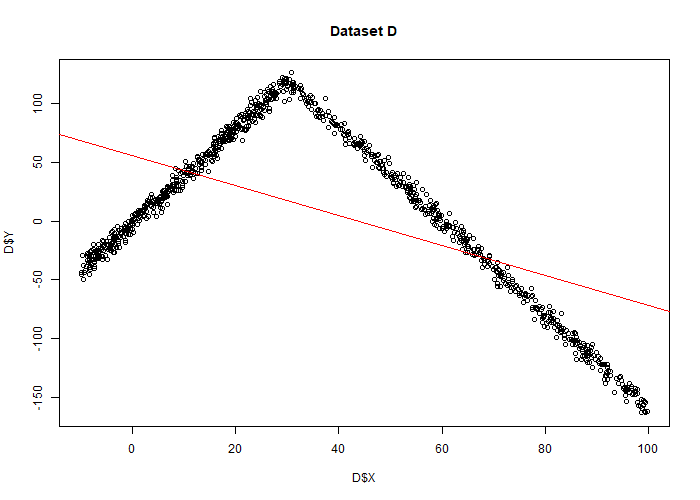
\includegraphics[width=0.48\textwidth]{figures/NuagePointD-DroiteRegression.png}
    \hfill
    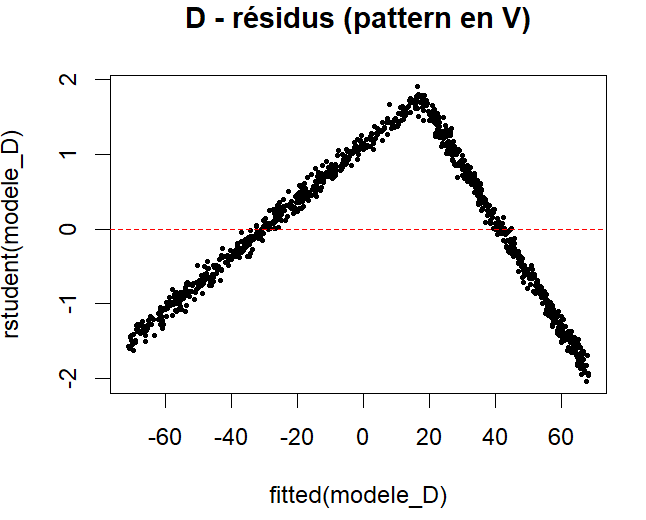
\includegraphics[width=0.48\textwidth]{figures/ResiduStudent-D.png}
    \caption{Ajustement linéaire direct, Dataset D.}
    \label{fig:D_simple}
\end{figure}

\subsubsection{Notre démarche : on coupe en deux}

En regardant le nuage, on voit que la pente change autour de $X = 30$. On coupe donc le jeu de données en deux et on fait une droite de chaque côté. Les diagnostics redeviennent corrects et les deux $R^2$ remontent (figure~\ref{fig:D_split}).

\begin{lstlisting}
D_g <- D[D$X < 30, ]
D_d <- D[D$X >= 30, ]
mod_g <- lm(Y ~ X, data = D_g)
mod_d <- lm(Y ~ X, data = D_d)
plot(D$X, D$Y, main = "deux droites")
abline(mod_g, col = "blue")
abline(mod_d, col = "red")
\end{lstlisting}

\begin{figure}[H]
    \centering
    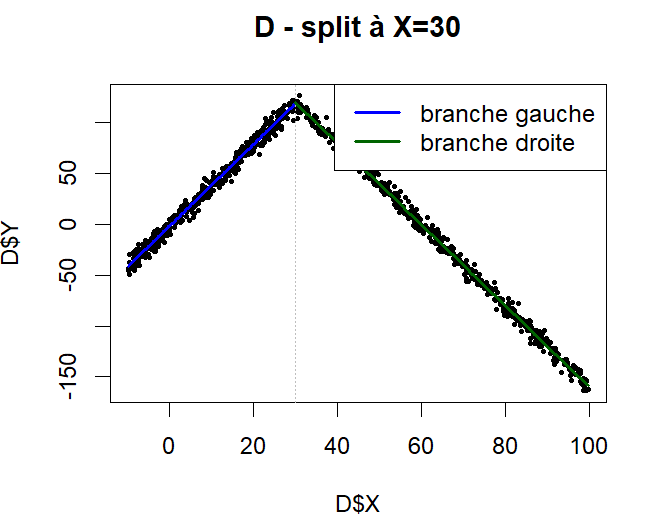
\includegraphics[width=0.7\textwidth]{figures/NuagePoint2droite-D.png}
    \caption{Deux droites séparées en $X = 30$, Dataset D.}
    \label{fig:D_split}
\end{figure}

\subsubsection{Apport de l'IA}

\begin{itemize}
    \item \textbf{Point de rupture estimé automatiquement.} Notre choix de $X = 30$ est fait à l'oeil. La régression segmentée (package \texttt{segmented}) estime le point de rupture $\hat{\psi}$ avec son erreur standard, donc le seuil devient une vraie estimation au lieu d'un choix arbitraire.

\begin{lstlisting}
library(segmented)
modele_D_seg <- segmented(modele_D, seg.Z = ~X, psi = 30)
cat("rupture estimee :", modele_D_seg$psi[, "Est."], "\n")
\end{lstlisting}

    \item \textbf{Modèle par morceaux en un seul \texttt{lm()}.} L'IA réécrit le tout avec une variable $Z = \max(X - 30, 0)$, ce qui est un cas particulier de régression multiple.

\begin{lstlisting}
D$Z <- pmax(D$X - 30, 0)
mod_pcw <- lm(Y ~ X + Z, data = D)
summary(mod_pcw)
\end{lstlisting}

    \item \textbf{Comparaison des $R^2$} entre le modèle simple (proche de 0) et le modèle segmenté (figure~\ref{fig:D_seg}).

\end{itemize}

\begin{figure}[H]
    \centering
    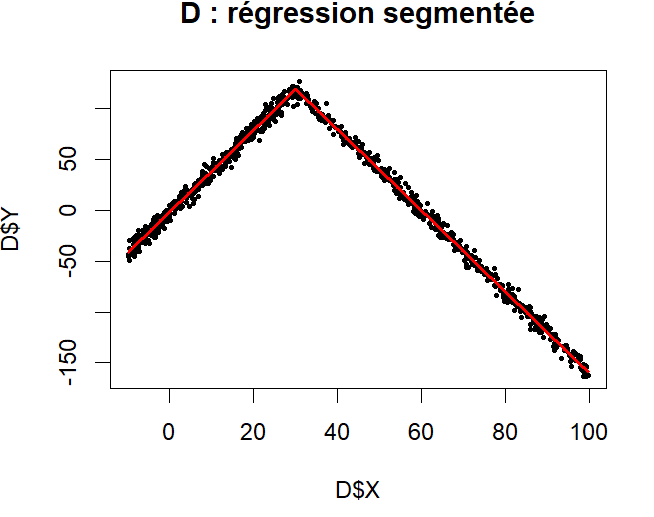
\includegraphics[width=0.7\textwidth]{figures/RegressionSegmente-D.png}
    \caption{Régression segmentée, Dataset D.}
    \label{fig:D_seg}
\end{figure}

%----------------------------------------------------------------------
\subsection{Bilan de la section}
%----------------------------------------------------------------------

Les quatre jeux correspondent à quatre situations classiques. Pour $A$ tout marche et on déroule la chaîne complète (ajustement, test, résidus, prédiction). Pour $B$ les moindres carrés sont sensibles aux points aberrants : on les enlève à la main, l'IA propose des méthodes plus robustes (rlm, distance de Cook). Pour $C$ la précision se dégrade avec le petit échantillon, et l'IA apporte des outils adaptés (bootstrap, erreurs robustes). Pour $D$ la droite ne convient pas : notre découpage manuel fonctionne mais l'IA le formalise avec la régression segmentée.

\newpage
%======================================================================
\section{Régression multiple, polynomiale et ANOVA}
%======================================================================

%----------------------------------------------------------------------
\subsection{Régression multiple}
%----------------------------------------------------------------------

On travaille sur le jeu $E$ qui a cinq variables explicatives $X_1, \dots, X_5$. Le modèle s'écrit sous forme matricielle $Y = X\beta + U$, et l'estimateur des moindres carrés est $\hat{\beta} = (X'X)^{-1}X'Y$. On juge le modèle avec le $R^2$ ajusté (qui pénalise le nombre de variables), le test de Fisher global (au moins une variable utile ?) et les tests de Student sur chaque coefficient.

\subsubsection{Notre démarche}

On ajuste le modèle complet et on lit le \texttt{summary()}. Le test de Fisher global est très significatif, donc le modèle apporte quelque chose. En regardant les p-valeurs une par une, on remarque que $X_2$ a une p-valeur trop grande. On regarde aussi \texttt{pairs()} et la matrice de corrélation pour voir les liens entre variables (figure~\ref{fig:mult_pairs}).

\begin{lstlisting}
modele_E <- lm(Y ~ X1 + X2 + X3 + X4 + X5, data = E)
summary(modele_E)
pairs(E)
cor(E)
\end{lstlisting}

\begin{figure}[H]
    \centering
    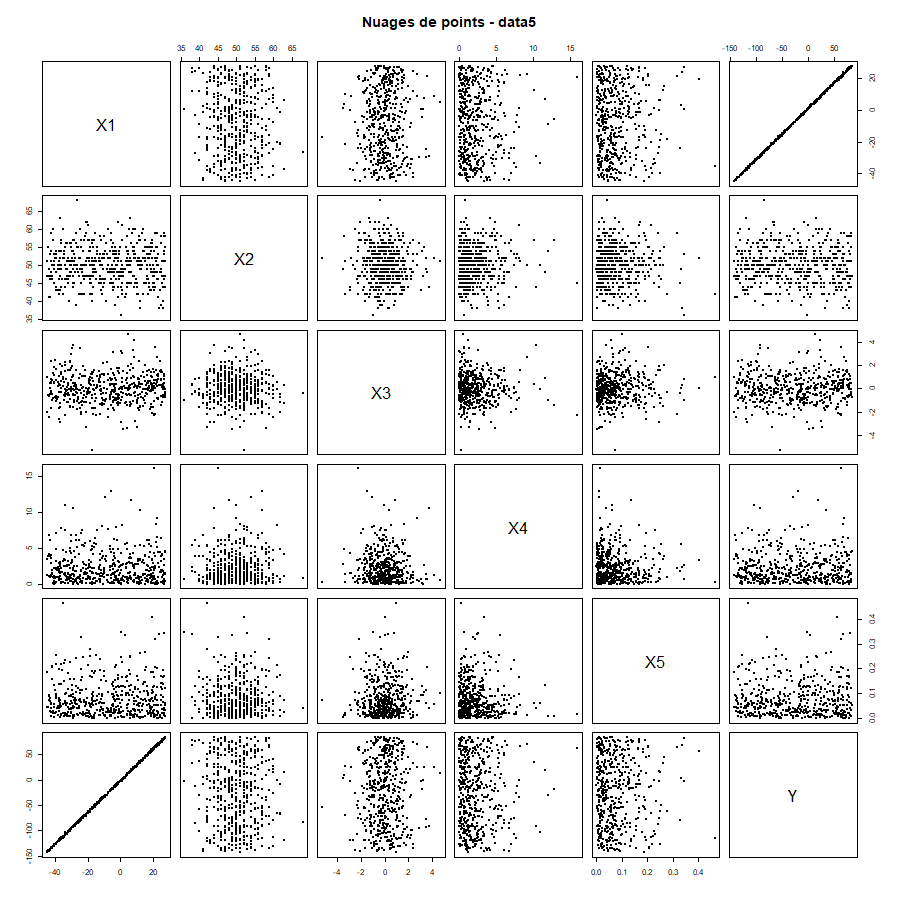
\includegraphics[width=0.7\textwidth]{figures/mult_pairs.png}
    \caption{Matrice des nuages de points entre les variables de $E$.}
    \label{fig:mult_pairs}
\end{figure}

Comme $X_2$ n'est pas significative, on l'enlève et on compare les deux modèles avec un test de Fisher (\texttt{anova}). La p-valeur est grande, donc on ne perd rien à retirer $X_2$ : on garde le modèle réduit. On vérifie enfin les résidus avec les graphiques de diagnostic (figure~\ref{fig:mult_diag}).

\begin{lstlisting}
modele_E2 <- lm(Y ~ X1 + X3 + X4 + X5, data = E)
anova(modele_E2, modele_E)

par(mfrow = c(2, 2))
plot(modele_E)
par(mfrow = c(1, 1))
\end{lstlisting}

\begin{figure}[H]
    \centering
    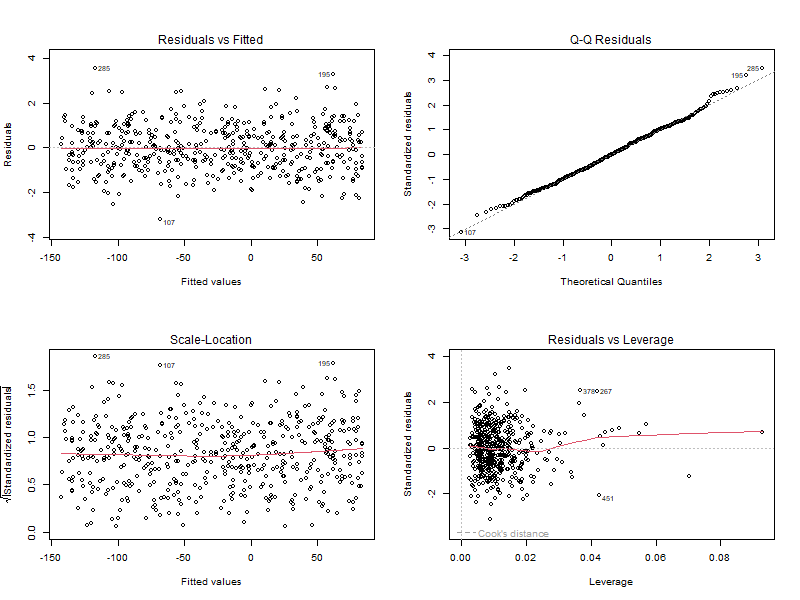
\includegraphics[width=0.8\textwidth]{figures/mult_diag.png}
    \caption{Diagnostics des résidus, régression multiple sur $E$.}
    \label{fig:mult_diag}
\end{figure}

\subsubsection{Apport de l'IA}

\begin{itemize}
    \item \textbf{Sélection automatique.} L'IA fait directement une sélection backward par AIC avec \texttt{step()}, ce qui retrouve le même modèle sans avoir à retirer les variables une par une à la main.

\begin{lstlisting}
modele_E_step <- step(modele_E, direction = "backward", trace = 0)
summary(modele_E_step)
\end{lstlisting}

    \item \textbf{Multicolinéarité (VIF).} L'IA calcule les VIF pour vérifier que les variables ne sont pas trop corrélées entre elles. Ici ils sont proches de 1, donc pas de problème.

\begin{lstlisting}
library(car)
vif(modele_E)
\end{lstlisting}

    \item \textbf{Test d'homoscédasticité.} En plus du graphique, l'IA confirme avec un test de Breusch-Pagan.

\begin{lstlisting}
library(lmtest)
bptest(modele_E)
\end{lstlisting}

\end{itemize}

%----------------------------------------------------------------------
\subsection{Régression polynomiale}
%----------------------------------------------------------------------

On utilise le jeu $D$. L'idée est qu'un modèle polynomial du type $Y = a X^2 + b X + c$ reste une régression multiple : il suffit de prendre $X$ et $X^2$ comme variables explicatives.

\subsubsection{Notre démarche}

On essaie d'abord une droite, qui marche mal. En comparant les corrélations, on voit que $Y$ est bien plus corrélé à $X^2$ qu'à $X$, donc on passe à un modèle quadratique. On trace la parabole sur le nuage (figure~\ref{fig:poly_main}).

\begin{lstlisting}
modele_lin   <- lm(Y ~ X, data = D)
cor(D$X, D$Y)
cor(D$X^2, D$Y)

modele_poly2 <- lm(Y ~ X + I(X^2), data = D)
plot(D$X, D$Y, main = "data4")
x_seq <- seq(min(D$X), max(D$X), length.out = 100)
lines(x_seq, predict(modele_poly2, data.frame(X = x_seq)), col = "red")
\end{lstlisting}

\begin{figure}[H]
    \centering
    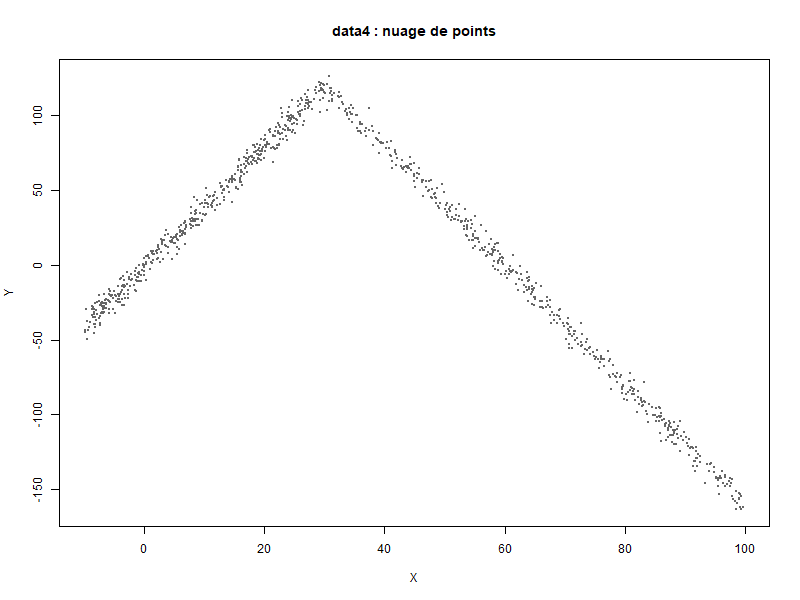
\includegraphics[width=0.48\textwidth]{figures/poly_scatter.png}
    \hfill
    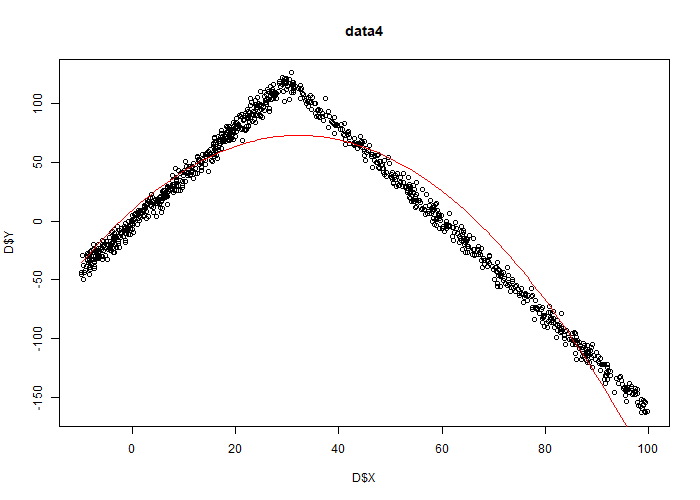
\includegraphics[width=0.48\textwidth]{figures/poly_fit.png}
    \caption{Nuage de points et ajustement quadratique, jeu $D$.}
    \label{fig:poly_main}
\end{figure}

On vérifie que le terme $X^2$ sert vraiment avec un test de Fisher entre le modèle linéaire et le modèle quadratique : la p-valeur est minuscule, donc $X^2$ est utile. Le $R^2$ passe d'une valeur faible à une valeur élevée, et les résidus sont bons (figure~\ref{fig:poly_diag}).

\begin{lstlisting}
anova(modele_lin, modele_poly2)
summary(modele_lin)$r.squared
summary(modele_poly2)$r.squared

par(mfrow = c(2, 2))
plot(modele_poly2)
par(mfrow = c(1, 1))
\end{lstlisting}

\begin{figure}[H]
    \centering
    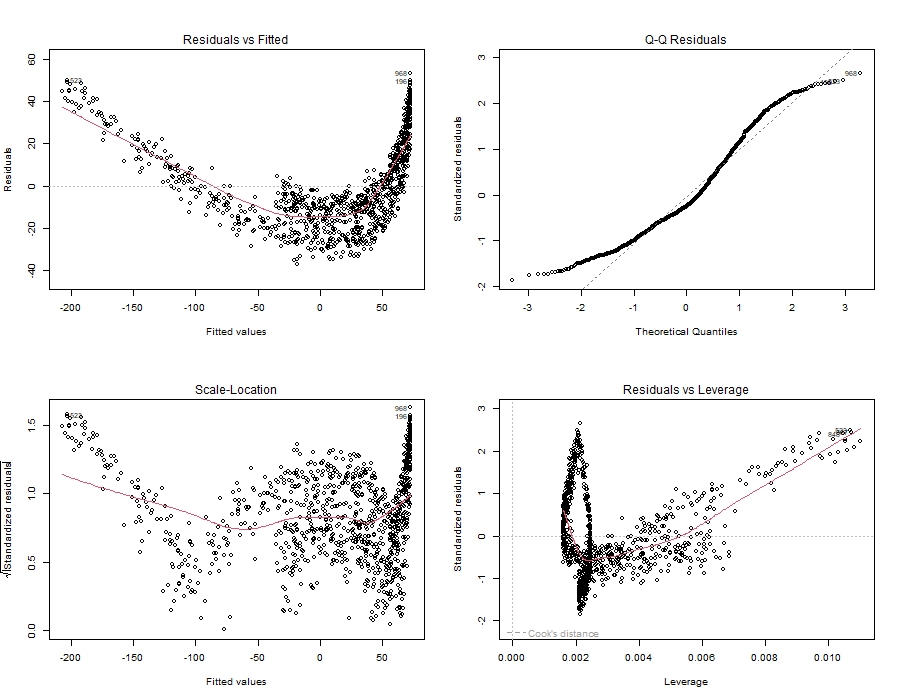
\includegraphics[width=0.8\textwidth]{figures/poly_diag.png}
    \caption{Diagnostics des résidus, modèle quadratique.}
    \label{fig:poly_diag}
\end{figure}

\subsubsection{Apport de l'IA}

\begin{itemize}
    \item \textbf{Choix du degré.} L'IA teste aussi les degrés 3 et 4 et les compare par AIC et par test de Fisher emboîté, pour vérifier qu'on ne gagne rien à monter plus haut que 2.

\begin{lstlisting}
modele_poly3 <- lm(Y ~ poly(X, 3, raw = TRUE), data = D)
modele_poly4 <- lm(Y ~ poly(X, 4, raw = TRUE), data = D)
cat("AIC deg.2 :", AIC(modele_poly2),
    "| deg.3 :", AIC(modele_poly3),
    "| deg.4 :", AIC(modele_poly4), "\n")
anova(modele_poly2, modele_poly3, modele_poly4)
\end{lstlisting}

    \item \textbf{Base orthogonale.} Pour les degrés élevés, l'IA utilise \texttt{poly(X, 3)} (base orthogonale) qui est plus stable numériquement que les puissances brutes.

\begin{lstlisting}
modele_poly_orth <- lm(Y ~ poly(X, 3), data = D)
summary(modele_poly_orth)
\end{lstlisting}

\end{itemize}

%----------------------------------------------------------------------
\subsection{ANOVA}
%----------------------------------------------------------------------

On utilise le jeu $G$. On fabrique deux facteurs : $F_1$ à partir de $X_6$ (déjà discret) et $F_2$ en découpant $X_7$ en trois classes. L'ANOVA revient à une régression linéaire avec des variables qualitatives.

\subsubsection{Notre démarche}

On regarde d'abord les moyennes par groupe et les boxplots (figure~\ref{fig:anova_main}, gauche). Puis on fait une ANOVA à un facteur sur chaque facteur, et une ANOVA à deux facteurs avec interaction. Le graphique d'interaction (figure~\ref{fig:anova_main}, droite) permet de voir si les courbes sont parallèles ou non.

\begin{lstlisting}
G$F1 <- factor(G$X6)
G$F2 <- cut(G$X7, breaks = c(-Inf, 6, 9, Inf), labels = c("bas", "moyen", "haut"))
tapply(G$Y, G$F1, mean)
boxplot(Y ~ F1, data = G)

aov_2f <- aov(Y ~ F1 * F2, data = G)
summary(aov_2f)
interaction.plot(G$F2, G$F1, G$Y)
\end{lstlisting}

\begin{figure}[H]
    \centering
    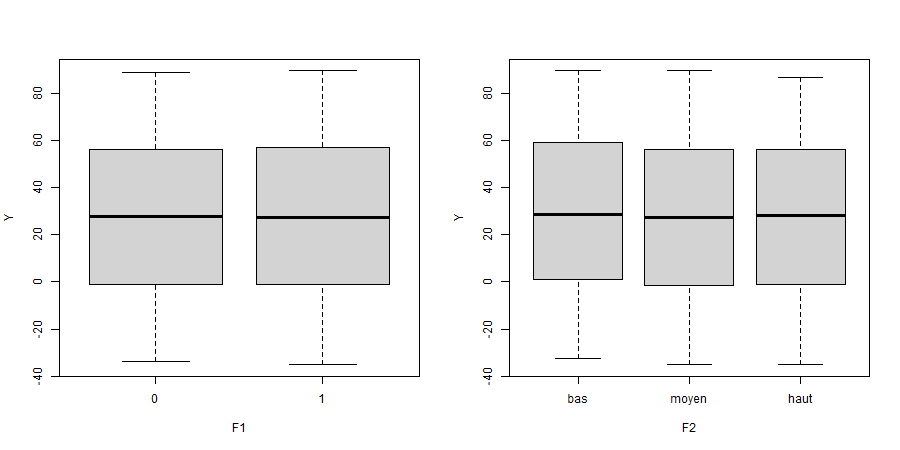
\includegraphics[width=0.48\textwidth]{figures/anova_boxplots.png}
    \hfill
    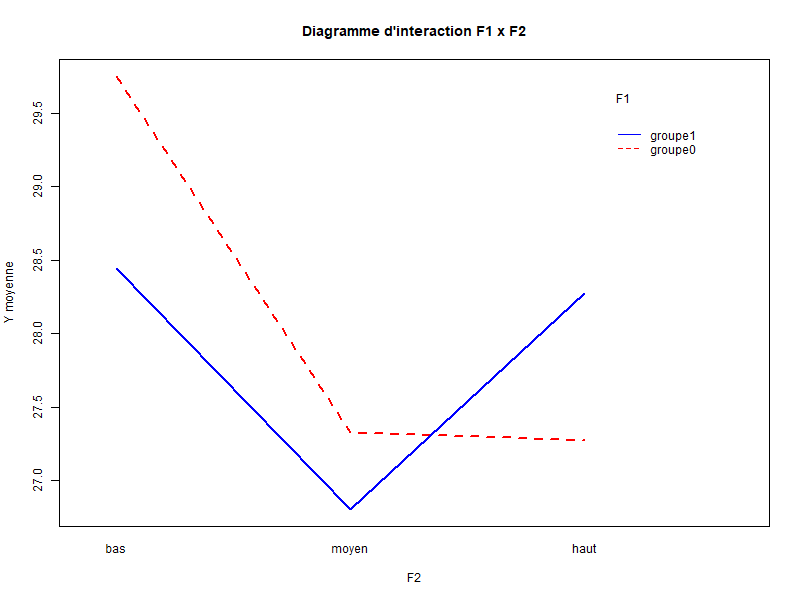
\includegraphics[width=0.48\textwidth]{figures/anova_interaction.png}
    \caption{Boxplots par groupe et graphique d'interaction, jeu $G$.}
    \label{fig:anova_main}
\end{figure}

On vérifie ensuite la normalité des résidus avec un QQ-plot (figure~\ref{fig:anova_diag}).

\begin{lstlisting}
qqnorm(rstudent(aov_2f))
qqline(rstudent(aov_2f))
\end{lstlisting}

\begin{figure}[H]
    \centering
    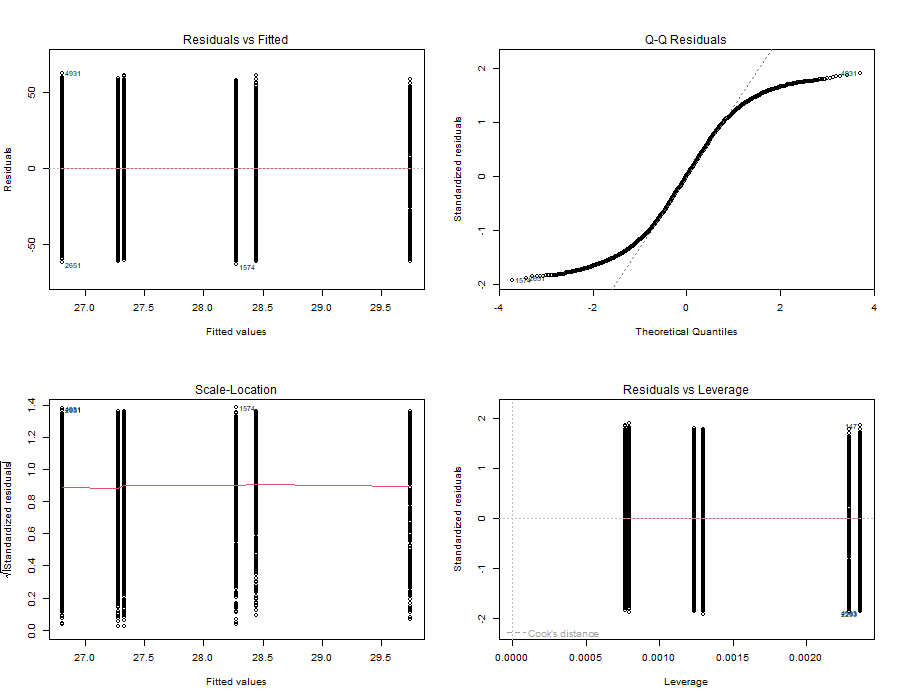
\includegraphics[width=0.6\textwidth]{figures/anova_diag.png}
    \caption{QQ-plot des résidus de l'ANOVA à deux facteurs.}
    \label{fig:anova_diag}
\end{figure}

\subsubsection{Apport de l'IA}

\begin{itemize}
    \item \textbf{Test post-hoc de Tukey.} L'ANOVA dit seulement qu'au moins un groupe diffère. L'IA ajoute le test de Tukey qui dit précisément quelles modalités diffèrent entre elles.

\begin{lstlisting}
TukeyHSD(aov_2f, which = "F2")
\end{lstlisting}

    \item \textbf{Garder la variable quantitative.} L'IA fait remarquer que découper $X_7$ en classes fait perdre de l'information, et propose de garder $X_7$ telle quelle dans une régression.

\begin{lstlisting}
modele_X7_quanti <- lm(Y ~ X6 + X7, data = G)
summary(modele_X7_quanti)
\end{lstlisting}

    \item \textbf{Test de Levene.} Pour l'égalité des variances, l'IA utilise le test de Levene, plus robuste que Bartlett quand les données ne sont pas tout à fait normales.

\begin{lstlisting}
library(car)
leveneTest(Y ~ F1, data = G)
\end{lstlisting}

\end{itemize}

\newpage
%======================================================================
\section{Sélection de variables}
%======================================================================

On dispose de trois jeux ($E$, $F$, $G$) avec cinq variables explicatives chacun. Le but est de choisir le meilleur sous-ensemble de variables : avec trop de variables on risque le sur-ajustement, avec trop peu on perd de l'information. On compare les modèles avec le $R^2$ ajusté et le critère AIC.

%----------------------------------------------------------------------
\subsection{Notre démarche}
%----------------------------------------------------------------------

On regarde d'abord la matrice de corrélation et le modèle complet. Ensuite on utilise \texttt{regsubsets()} (package \texttt{leaps}), qui donne pour chaque taille de modèle le meilleur sous-ensemble de variables. On trace le $R^2$ ajusté en fonction du nombre de variables et on prend le maximum (figure~\ref{fig:select_E}).

\begin{lstlisting}
library(leaps)
cor(E)
complet_E <- lm(Y ~ X1 + X2 + X3 + X4 + X5, data = E)

sel_E <- regsubsets(Y ~ X1 + X2 + X3 + X4 + X5, data = E)
summary(sel_E)$which
summary(sel_E)$adjr2
which.max(summary(sel_E)$adjr2)
plot(summary(sel_E)$adjr2, type = "b", xlab = "nb variables", ylab = "R2 ajuste")
\end{lstlisting}

\begin{figure}[H]
    \centering
    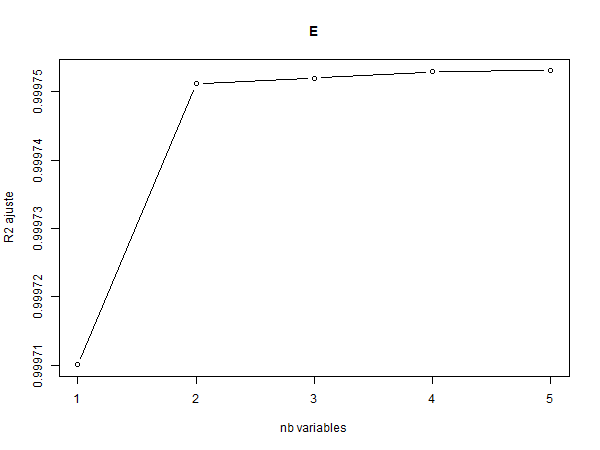
\includegraphics[width=0.6\textwidth]{figures/select_adjr2_E.png}
    \caption{$R^2$ ajusté en fonction du nombre de variables, jeu $E$.}
    \label{fig:select_E}
\end{figure}

On refait la même chose avec les méthodes pas à pas forward et backward, pour vérifier qu'elles donnent le même modèle que la recherche sur tous les sous-ensembles.

\begin{lstlisting}
sel_E_f <- regsubsets(Y ~ X1 + X2 + X3 + X4 + X5, data = E, method = "forward")
sel_E_b <- regsubsets(Y ~ X1 + X2 + X3 + X4 + X5, data = E, method = "backward")
summary(sel_E_f)$which
summary(sel_E_b)$which
\end{lstlisting}

On applique exactement la même démarche aux jeux $F$ et $G$ (figure~\ref{fig:select_FG}). Le $R^2$ ajusté atteint son maximum pour un sous-ensemble qui n'utilise pas toutes les variables, ce qui confirme qu'il faut bien en retirer certaines.

\begin{figure}[H]
    \centering
    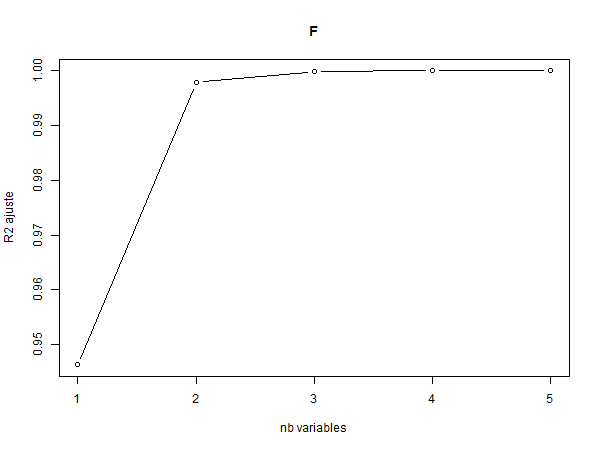
\includegraphics[width=0.48\textwidth]{figures/select_adjr2_F.png}
    \hfill
    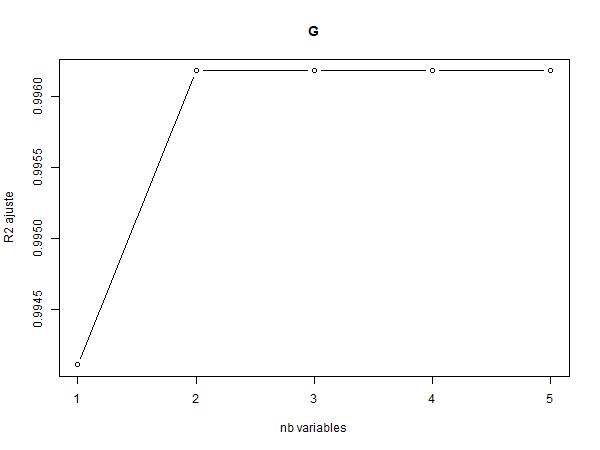
\includegraphics[width=0.48\textwidth]{figures/select_adjr2_G.png}
    \caption{$R^2$ ajusté en fonction du nombre de variables, jeux $F$ (gauche) et $G$ (droite).}
    \label{fig:select_FG}
\end{figure}

%----------------------------------------------------------------------
\subsection{Apport de l'IA}
%----------------------------------------------------------------------

\begin{itemize}
    \item \textbf{Sélection par AIC avec \texttt{step()}.} Le $R^2$ ajusté n'est qu'un critère parmi d'autres. L'IA fait la sélection avec \texttt{step()} basé sur l'AIC, dans les trois directions (backward, forward, both), et on compare les modèles obtenus.

\begin{lstlisting}
step_back_E <- step(complet_E, direction = "backward", trace = 0)
step_forw_E <- step(lm(Y ~ 1, data = E), direction = "forward",
                    scope = formula(complet_E), trace = 0)
step_both_E <- step(complet_E, direction = "both", trace = 0)
cat("backward :", paste(names(coef(step_back_E))[-1], collapse = " + "),
    "| AIC =", round(AIC(step_back_E), 1), "\n")
\end{lstlisting}

    \item \textbf{Multicolinéarité (VIF).} L'IA vérifie avec les VIF que les variables retenues ne sont pas redondantes entre elles, ce qui rendrait les coefficients instables.

\begin{lstlisting}
library(car)
vif(complet_E)
\end{lstlisting}

    \item \textbf{Homoscédasticité.} Comme dans les autres sections, l'IA ajoute un test de Breusch-Pagan sur le modèle retenu.

\begin{lstlisting}
library(lmtest)
bptest(complet_E)
\end{lstlisting}

\end{itemize}

\newpage
\section*{Conclusion}

Sur l'ensemble du projet, notre démarche d'étudiants nous a permis de traiter correctement tous les cas : ajuster un modèle, lire les sorties de R, vérifier les hypothèses avec les résidus et les tests, repérer les problèmes (points aberrants, non-linéarité, variables inutiles) et y réagir. L'IA, elle, n'a presque jamais changé nos conclusions, mais elle a systématiquement apporté des outils en plus : des tests formels pour objectiver les diagnostics graphiques (Breusch-Pagan, Shapiro, Levene), des méthodes plus robustes que la suppression manuelle (régression robuste, distance de Cook, bootstrap, erreurs sandwich), et de l'automatisation pour les choix qu'on faisait à la main (régression segmentée, \texttt{step()} par AIC). En résumé, l'IA ne remplace pas le raisonnement statistique mais elle élargit la boîte à outils et fiabilise les conclusions.

\end{document}
